% ==========================================
% فایل: steps/step02.tex
% گام ۲: محاسبه توصیف‌گرها و یافتن شبیه‌ترین نقاط
% ==========================================

\section{گام (۲): محاسبه توصیف‌گرها و یافتن شبیه‌ترین نقاط}

\begin{stepbox}
\field{روند کار و منطق ریاضی}{
پس از استخراج نقاط کلیدی توسط الگوریتم \lr{SIFT}، نیاز داریم تا هویت هر نقطه را به صورت ریاضی توصیف کنیم. به همین منظور برای هر نقطه یک بردار ویژگی ۱۲۸ بعدی (\lr{Descriptor}) محاسبه شد. 
برای سنجش دقیق شباهت بین این بردارها، از مفهوم «شباهت کسینوسی» (\lr{Cosine Similarity}) استفاده می‌کنیم. در برنامه‌نویسی، سریع‌ترین راه برای محاسبه‌ی شباهت کسینوسی این است که ابتدا طول تمام بردارها را به ۱ برسانیم (نرمال‌سازی) و سپس آن‌ها را در هم ضرب داخلی (\lr{Dot Product}) کنیم.
}

\begin{codebox}[محاسبه توصیف‌گر و نرمال‌سازی]
\begin{lstlisting}[language=Python]
# Compute 128-D SIFT descriptors for each keypoint
kp1_sift, des1 = sift.compute(img1_gray, kp1_sift)
kp2_sift, des2 = sift.compute(img2_gray, kp2_sift)

# Apply L2 Normalization to make vector lengths equal to 1
des1_norm = des1 / np.linalg.norm(des1, axis=1, keepdims=True)
des2_norm = des2 / np.linalg.norm(des2, axis=1, keepdims=True)
\end{lstlisting}
\end{codebox}

\field{یافتن بالاترین شباهت (کد و تحلیل)}{
به جای استفاده از حلقه‌های تو در تو که زمان‌بر هستند، با استفاده از جبر خطی و ضرب ماتریسی در کتابخانه‌ی \lr{NumPy}، شباهت تمام نقاطِ تصویر اول با تمام نقاطِ تصویر دوم را در کسری از ثانیه محاسبه کردیم. 
سپس با یافتن اندیسِ بزرگترین عدد در این ماتریس (\lr{Maximum Value})، شبیه‌ترین جفت‌نقطه استخراج شد.
}

\begin{codebox}[محاسبه ماتریس شباهت]
\begin{lstlisting}[language=Python]
# Calculate similarity matrix using dot product
similarity_matrix = np.dot(des1_norm, des2_norm.T)

# Find the 2D indices of the maximum similarity value
max_idx = np.unravel_index(np.argmax(similarity_matrix), similarity_matrix.shape)
idx1, idx2 = max_idx
\end{lstlisting}
\end{codebox}

\field{تحلیل بصری خروجی‌ها در مجموعه‌های مختلف}{
با رسم خط متصل‌کننده بین این دو نقطه (\lr{Highest Similarity Match}) در سه مجموعه‌ی تصویری مختلف، دقت الگوریتم اثبات می‌شود:
\begin{itemize}
    \item \textbf{در مجموعه اول (\lr{Set 1}):} شبیه‌ترین نقطه دقیقاً بر روی گوشه‌ی تاریک شیار دستگاه پرینتر/تجهیزات تشخیص داده شده است که کنتراست بالایی دارد.
    \item \textbf{در مجموعه دوم (\lr{Set 2}):} نقطه بر روی لبه‌ی پله‌های سنگی در مرکز تصویر مچ شده است که دارای ساختار هندسی بسیار پایداری در هر دو زاویه دید است.
    \item \textbf{در مجموعه سوم (\lr{Set 3}):} الگوریتم موفق شده یک نقطه‌ی متمایز از بافت تکرارشونده‌ی موکت کف اتاق را با دقت بالا در هر دو تصویر شناسایی کند.
\end{itemize}
}
\end{stepbox}

\begin{figure}[h!]
    \centering
    \begin{subfigure}{0.48\textwidth}
        \centering
        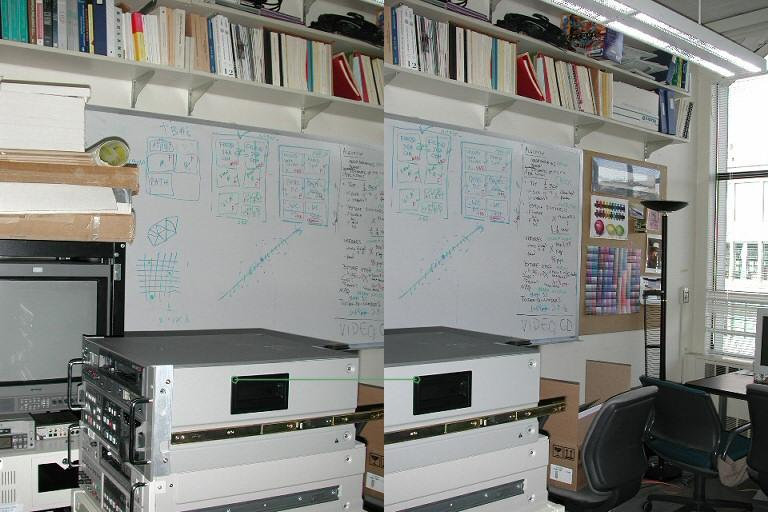
\includegraphics[width=\textwidth]{images/Part_2/Highest_Similarity_Match_set1.jpg}
        \caption{مجموعه اول: تطابق بر روی لبه‌ی تجهیزات}
    \end{subfigure}
    \hfill
    \begin{subfigure}{0.48\textwidth}
        \centering
        
\includegraphics[width=\textwidth]{images/Part_2/Highest_Similarity_Match.jpg}
        \caption{مجموعه دوم: تطابق بر روی ساختار پله‌ها}
    \end{subfigure}
    
    \vspace{0.4cm}
    \begin{subfigure}{0.6\textwidth}
        \centering
        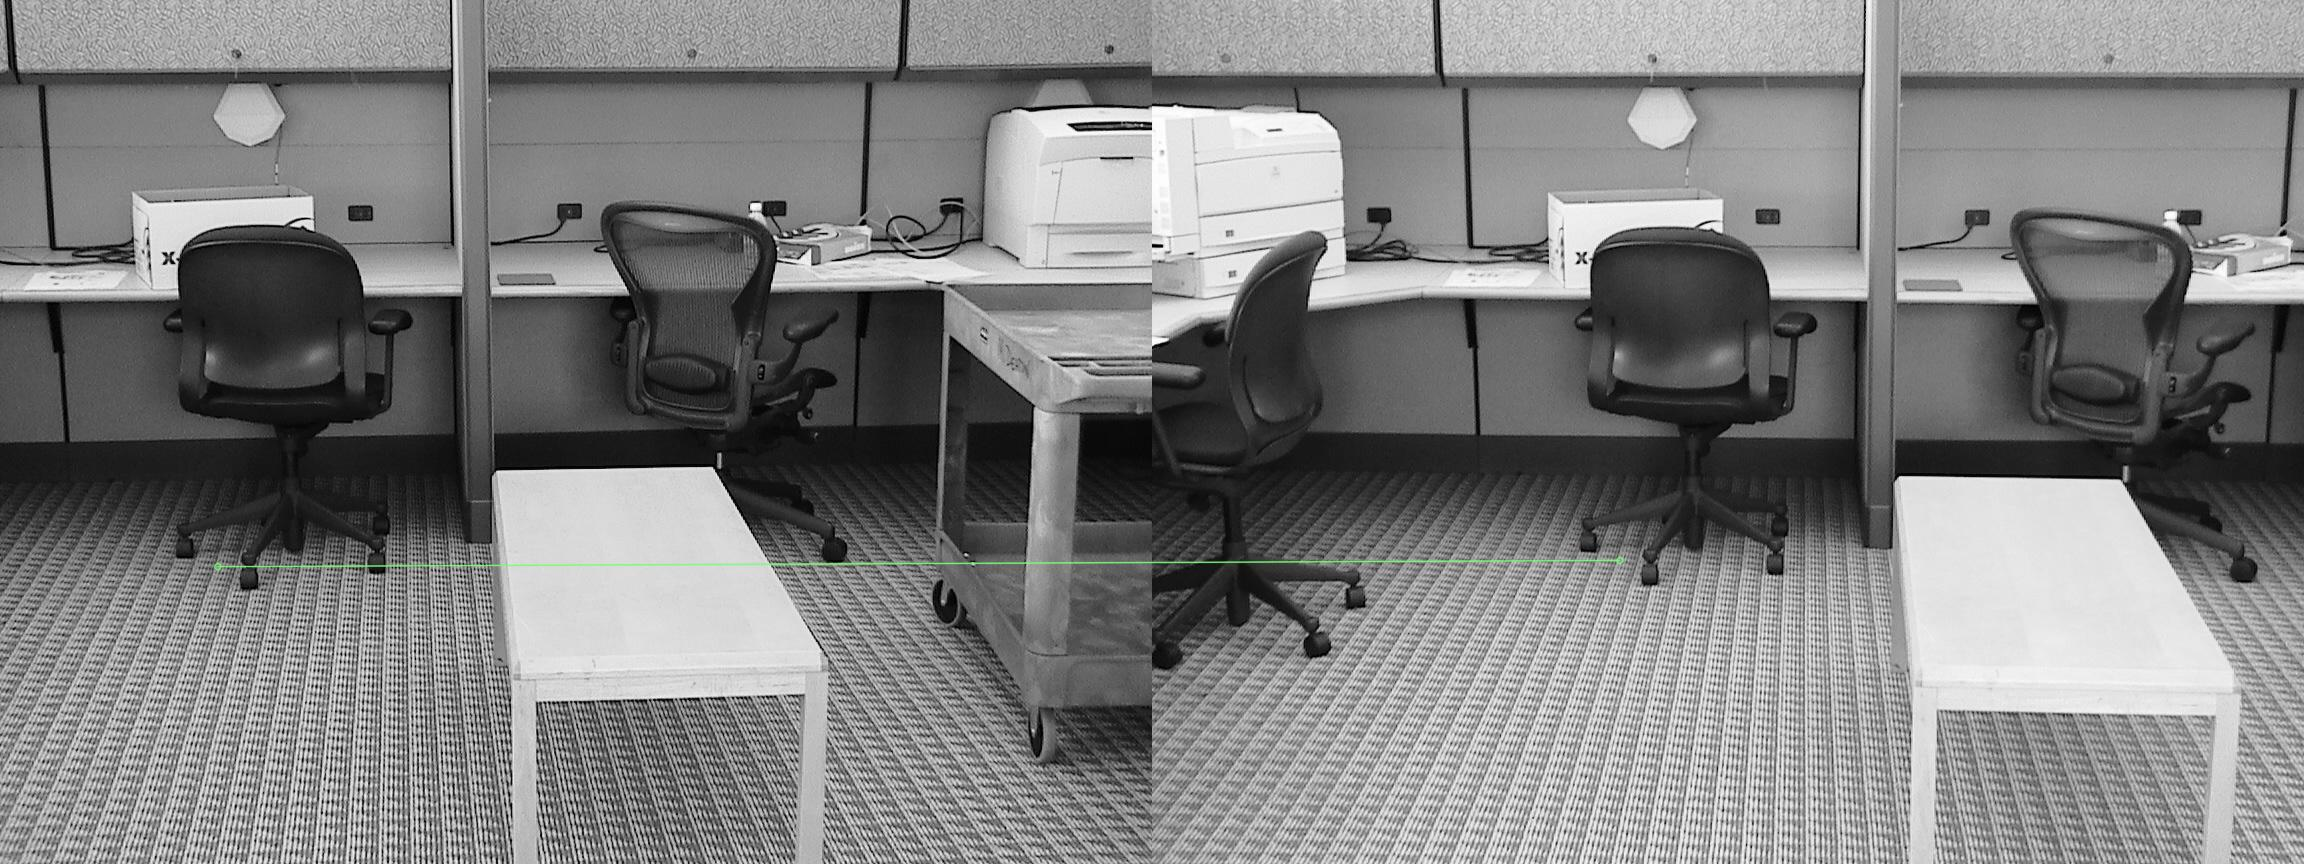
\includegraphics[width=\textwidth]{images/Part_2/Highest_Similarity_Match_set3.jpg}
        \caption{مجموعه سوم: تطابق دقیق بر روی بافت موکت}
    \end{subfigure}
    \caption{بررسی عملکرد الگوریتم در یافتن شبیه‌ترین نقاط کلیدی در شرایط محیطی متفاوت}
\end{figure}